\documentclass[aspectratio=169,11pt]{beamer}

% Shared style (ib-tutorials.sty at the repo root).
\makeatletter\def\input@path{{./}{../}}\makeatother
\usepackage{ib-tutorials}

\usepackage[utf8]{inputenc}
\usepackage{amsmath,amssymb}
\usepackage{booktabs}
\usepackage{array}
\newcolumntype{L}[1]{>{\raggedright\arraybackslash}p{#1}}
\usepackage{graphicx}
\graphicspath{{../pictures/1-getting-set-up/}{../pictures/2-ib2d/}{../pictures/3-ibamr-fundamentals/}{../pictures/4-ibfe/}{../pictures/5-visit/}{../pictures/planktos/}{../examples/IB/13-carotid-bifurcation/}}
\usepackage{xcolor}
\usepackage{listings}
\usepackage{tikz}
\usetikzlibrary{arrows.meta,positioning,shapes.geometric,fit,calc}
\usepackage{hyperref}

\newcommand{\sourcecredit}[1]{\vfill\begin{flushright}\tiny\textcolor{DarkGray}{#1}\end{flushright}}
\newcommand{\gui}[1]{\textsf{\textbf{#1}}}
% One example per page: picture left, the facts right.
\newcommand{\expic}[2]{\centering\includegraphics[width=\linewidth,height=0.6\textheight,keepaspectratio]{#1}\par\vspace{1mm}{\tiny\color{DarkGray}#2\par}}

\lstset{
  basicstyle=\ttfamily\scriptsize\color{BlackGray},
  keywordstyle=\color{NavyBlue}\bfseries,
  commentstyle=\color{DarkGray}\itshape,
  stringstyle=\color{OliveGreen},
  showstringspaces=false,
  columns=fullflexible,
  keepspaces=true,
  breaklines=true,
  breakindent=1em,
  frame=single,
  framerule=0.4pt,
  rulecolor=\color{LightGray},
  backgroundcolor=\color{LightGray!30},
  xleftmargin=0.25em,
  xrightmargin=0.25em
}
\lstdefinestyle{shell}{morecomment=[l]{\#}}

\title[Catalogue of examples]{Catalogue of examples}
\subtitle{One page per example of this series: what it models, how to run it, what you should see, what to try, and where the chapters explain it}
\author[Miller]{Laura A. Miller}
\institute[UArizona]{Department of Mathematics, University of Arizona}
\date{Using IB Software \textbullet\ Part VII \textbullet\ Chapter 36}

\begin{document}

% 1
\begin{frame}[plain]
\maketutorialtitlepanel{%
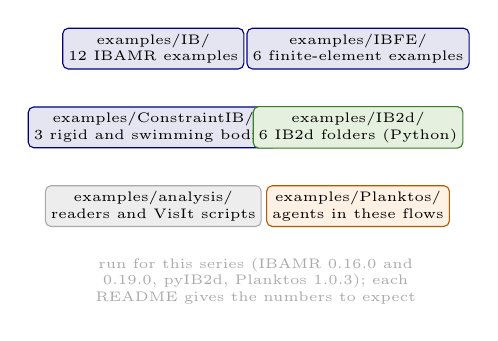
\begin{tikzpicture}[every node/.style={font=\tiny}, box/.style={draw, rounded corners=2pt, align=center, inner sep=2pt, minimum width=2.2cm}]
  \node[box,draw=NavyBlue,fill=NavyBlue!10] at (0,1.5) {\code{examples/IB/}\\12 IBAMR examples};
  \node[box,draw=NavyBlue,fill=NavyBlue!10] at (2.6,1.5) {\code{examples/IBFE/}\\6 finite-element examples};
  \node[box,draw=NavyBlue,fill=NavyBlue!10] at (0,0.5) {\code{examples/ConstraintIB/}\\3 rigid and swimming bodies};
  \node[box,draw=OliveGreen,fill=OliveGreen!10] at (2.6,0.5) {\code{examples/IB2d/}\\6 IB2d folders (Python)};
  \node[box,draw=DarkGray,fill=LightGray!40] at (0,-0.5) {\code{examples/analysis/}\\readers and VisIt scripts};
  \node[box,draw=orange!70!black,fill=orange!10] at (2.6,-0.5) {\code{examples/Planktos/}\\agents in these flows};
  \node[text=DarkGray,align=center,text width=5cm] at (1.3,-1.45) {run for this series (IBAMR 0.16.0 and 0.19.0, pyIB2d, Planktos 1.0.3); each README gives the numbers to expect};
\end{tikzpicture}}
\end{frame}

% 2
\begin{frame}{Learning goals}
\label{fr:goals}
By the end of this chapter you should be able to:
\begin{enumerate}
  \item find the example closest to the model you want to build, and the chapters that explain it;
  \item build and run any IBAMR example of this series on your computer or on Puma, and any pyIB2d example;
  \item check a run against the numbers its README gives, before you change anything;
  \item know what each example's ``things to try'' will teach you, and which of them break the run on purpose.
\end{enumerate}
\begin{punchbox}
\small Start from the example nearest to your problem, run it unchanged, compare with its README, then change one thing at a time.
\end{punchbox}
\end{frame}

% 3
\begin{frame}{The examples at a glance (1/2): IBAMR's IB method}
\label{fr:glance1}
\scriptsize
\renewcommand{\arraystretch}{0.95}
\begin{tabular}{@{}L{0.24\textwidth}L{0.40\textwidth}L{0.10\textwidth}L{0.16\textwidth}@{}}
\toprule
example & what it shows & run & chapters \\
\midrule
IB/01 rubber band & springs; an ellipse relaxes to a circle & 3--4 min, 4 cores & 3, 6, 26 \\
IB/02 pulsatile channel & target-point walls; pulsing inflow & 5--6 min, 4 & 7, 6, 3 \\
IB/03 tethered beam & a leaf bending in a flow; beams & 7 min, 4 & 7, 6, 10 \\
IB/04 moving cylinders & moving target points; drag & 6 min, 4 & 9a, 6, 11 \\
IB/06 growing springs & rest lengths that change; folding & 3 min, 4 & 9a, 6, 10 \\
IB/07 moving plates & two structures pulled apart & 5--8 min, 4 & 9a, 6, 11 \\
IB/08 glycocalyx in 3D & a fibre in a sheared box; 3D & 20 min, 4 & 12, 7, 9a, 27 \\
IB/09 curling beam & preferred curvature in time & 12 min, 3 & 10, 9a, 6, 11 \\
IB/10 jellyfish bell & a free body that swims by curvature & 15 min, 2 & 10, 9a, 6, 8b, 11 \\
IB/11 heart-tube pump & five ways to drive a valveless pump & 40--86 min per mode, 3 (five at once) & 9b, 9a, 6, 11, 29, 30 \\
IB/12 spider ballooning & a massive point (penalty IB); gravity & 20 min, 3 & 13, 6, 8b, 11 \\
IB/13 carotid, horse and human & real vessels; pulsatile inflow, open outflow & 3.5 and 44 min, 4 & 7, 6, 8a, 11, 25, 26 \\
\bottomrule
\end{tabular}

\vspace{1mm}
\footnotesize There is no IB/05 in the public repository. Times: a desktop PC under WSL, on the cores shown; every \code{job.slurm} asks for 4 (IB/13's for 16).
\sourcecredit{The examples' \code{README.md} files (October 2026).}
\end{frame}

% 4
\begin{frame}{The examples at a glance (2/2): IBFE, ConstraintIB, IB2d, analysis, Planktos}
\label{fr:glance2}
\scriptsize
\renewcommand{\arraystretch}{0.95}
\begin{tabular}{@{}L{0.26\textwidth}L{0.39\textwidth}L{0.11\textwidth}L{0.14\textwidth}@{}}
\toprule
example & what it shows & run & chapters \\
\midrule
IBFE/01 tethered plate & a finite-element plate on a tether, three motions & under 1 min & 17, 19, 28 \\
IBFE/05 gmsh triangle & a mesh from gmsh & 2 min & 18, 17, 28 \\
IBFE/06 active tension & a muscle-like active stress & under 1 min & 20, 19, 28 \\
IBFE/08 plate hits circle & two meshes (parts) & 2 min & 21, 18, 28 \\
IBFE/10 flow tank (3D) & a plate in a 3D stream & 30--50 min & 22, 18, 19, 27, 28 \\
IBFE/12 advection--diffusion & a scalar stirred by the plate & 1.5 min & 24, 7, 28 \\
ConstraintIB/01--03 & a prescribed cylinder, a free cylinder, a swimming eel & 2.5--12 min & 14, 15 \\
IB2d: 6 folders & moving targets, a pump, a heart, the stability lab, muscle laws, meshes from SVG & seconds to hours & 4c--4f \\
\code{analysis/} & readers (Python, MATLAB/Octave), VisIt scripts, a Slurm job & -- & 11, 27--33, 35 \\
\code{Planktos/} & agents in this series' flows & seconds to minutes & 34, 35 \\
\code{support/} & the course's MATLAB exercises with Python versions & -- & 5, 4d, 16; Appendix A \\
\bottomrule
\end{tabular}

\vspace{1mm}
\footnotesize IBFE runs on 4 cores, ConstraintIB on 4 or 8 ranks (timed with the three running at once); IB2d examples run in Python (one process).
\sourcecredit{The examples' \code{README.md} files (October 2026).}
\end{frame}

% 5
\begin{frame}[fragile]{How every IBAMR example runs}
\label{fr:howibamr}
\begin{lstlisting}[style=shell]
module load gnu13 openmpi5                       # on Puma, inside a job (chapter 1); not on your own computer
source ~/autoibamr/configuration/enable.sh       # IBAMR built by autoibamr (chapter 2)
cmake -S . -B build -DCMAKE_BUILD_TYPE=Release   # in the example's folder
cmake --build build -j 4
mpirun -np 4 ./build/main2d input2d              # main3d input3d for IB/08 and IBFE/10
sbatch job.slurm                                 # or this, on Puma (set your group in it first)
\end{lstlisting}
\footnotesize
\begin{itemize}\setlength{\itemsep}{1pt}
  \item Each folder holds \code{main.cpp} (and any update functions), the structure files or the mesh, the input file, \code{CMakeLists.txt}, \code{job.slurm} and a \code{README.md}: files, the physics, build and run, what you should see, looking at it in VisIt, things to try, history.
  \item Input files must keep Unix line endings: an edit on Windows gives \code{Illegal character token in input} (\code{dos2unix input2d}; the repository's \code{.gitattributes} checks them out right).
\end{itemize}
\sourcecredit{The examples' \code{README.md} files; chapters 1--3.}
\end{frame}

% 5b
\begin{frame}{How every IBAMR example runs (2)}
\label{fr:howibamr2}
\footnotesize
\begin{itemize}\setlength{\itemsep}{1pt}
  \item An example with an update function or a kinematics class lists every source in \code{CMakeLists.txt} (IB/04, 06--11, ConstraintIB/01--03); if one is missing, the link fails with \code{undefined reference to \dots}.
  \item IB/11 has one input file per mode (\code{input2d}, \code{input2d.force-vp}, \dots; its \code{job.slurm} runs \code{input2d}: change the name on its last line), IB/13 one per case (\code{input2d.human}, \code{input2d.horse}; its \code{job.slurm} runs the horse at twice the resolution on 16 cores).
  \item Tested with IBAMR 0.16.0 and 0.19.0 (autoibamr; GCC 13.3, Open MPI 4.1.6, Ubuntu 24.04); IB/13 and ConstraintIB with 0.19.0.
\end{itemize}
\sourcecredit{The examples' \code{README.md} and \code{job.slurm} files; chapters 1--3.}
\end{frame}

% 6
\begin{frame}[fragile]{How the IB2d examples run}
\label{fr:howib2d}
\begin{lstlisting}[style=shell]
git clone https://github.com/nickabattista/IB2d.git        # once (chapter 4a)
cp -r examples/IB2d/Pulsing_Heart IB2d/pyIB2d/Examples/    # main2d.py finds ../../IBM_Blackbox from there
cd IB2d/pyIB2d/Examples/Pulsing_Heart
python3 main2d.py                                          # writes viz_IB2d/ (VTK) for VisIt (chapter 4b)
\end{lstlisting}
\footnotesize
\begin{itemize}\setlength{\itemsep}{1pt}
  \item The four pyIB2d folders (\code{Moving\_Rubberband}, \code{Sawtooth}, \code{Pulsing\_Heart}, \code{Stability\_Lab}) and \code{Mesh\_From\_SVG/Starfish\_Channel} are ports of IB2d's MATLAB examples or the shipped Python ones, with generators that write the structure files (\code{Pulsing\_Heart} ships the MATLAB example's files, its two shapes as data, instead); the indices in the structure files are 0-based in pyIB2d.
  \item \code{Muscle\_Models} needs only NumPy and Matplotlib; \code{Mesh\_From\_SVG/svg\_to\_vertex.py} only NumPy.
  \item IB2d's own files and line-for-line ports of its code stay GPL-3.0 and say so in their headers: the \code{main2d.py} of \code{Stability\_Lab} and \code{Starfish\_Channel}, \code{Starfish\_Channel}'s forcing, \code{activation\_wave.py} and \code{calcium\_activation.py}; the other \code{main2d.py} files are this repository's code.
\end{itemize}
\sourcecredit{\code{examples/IB2d/README.md} and the folders' READMEs; chapters 4a--4f.}
\end{frame}

% 7
\begin{frame}{IB/01 Rubber band}
\label{fr:ib01}
\begin{columns}[T,onlytextwidth]
\column{0.42\textwidth}
\expic{ch5-rubber-band-omega.png}{The band and the vorticity around it at $t = 0.12$ s (chapter 5 shows it with the refined patches).}
\column{0.55\textwidth}
\scriptsize
\al{What:} 644 points joined by springs start as an ellipse (semi-axes 0.12 and 0.10 m) in a periodic box of fluid ($\rho = 1000$, $\mu = 100$) and relax into a circle. The springs' rest length is that of a circle of radius 0.1 m, but the fluid inside cannot escape: the band ends as a circle of radius $\sqrt{0.12 \times 0.10} \approx 0.1095$ m.

\smallskip
\al{Run:} 20,000 steps; about 3--4 minutes on 4 cores (166 s with IBAMR 0.16.0, 181 s with 0.19.0; 4 min 14 s as a batch job on Puma).

\smallskip
\al{You should see:} \code{integral\{F\}} at round-off every 400 steps (the springs' forces cancel in pairs); width/height 1.200 at the start, 0.996 at $t = 0.4$ s (a slight overshoot), 1.000 from 1 s on.

\smallskip
\al{Try:} \code{MU = 10} or 1: the band swings between wide and tall about once every 0.3 s; \code{DT = 1.0e-3}: \code{Time step size change encountered} (chapter 16).

\smallskip
\al{Chapters:} 3 (building and running), 6 (structure files), 26 (VisIt); 5 and 8a use it too.
\end{columns}
\sourcecredit{\code{examples/IB/01-rubber-band/README.md}.}
\end{frame}

% 8
\begin{frame}{IB/02 Pulsatile channel}
\label{fr:ib02}
\begin{columns}[T,onlytextwidth]
\column{0.42\textwidth}
\expic{ch7-channel-peak-speed.png}{The speed at the peak of the inflow (chapter 7).}
\column{0.55\textwidth}
\scriptsize
\al{What:} fluid pulses through a straight channel (width 1) whose walls are rows of target points; the inflow and outflow are parabolas whose peak pulses between 0 and 1 at 5 Hz, written as muParser expressions. A $5\times5$ box, not periodic, 3 levels (512 cells across the finest); springs and beams of stiffness $10^{-10}$ only show the file formats.

\smallskip
\al{Run:} 20,000 steps, 51 frames (49 MB); about 5--6 minutes on 4 cores (318 s with IBAMR 0.16.0).

\smallskip
\al{You should see:} \code{integral\{F\}}, the force holding the walls, negative in $x$ and pulsing with the inflow, and growing from cycle to cycle: momentum takes $\rho d^2/\mu = 10$ s to cross the channel, so the flow is still developing.

\smallskip
\al{Try:} another frequency \code{f}; a steady inflow (replace the pulse by 1.0) run until the profile settles; a longer \code{END\_TIME}, until the force repeats.

\smallskip
\al{Chapters:} 7 (boundary conditions), 6 (structure files), 3 (input-file errors).
\end{columns}
\sourcecredit{\code{examples/IB/02-pulsatile-channel/README.md}.}
\end{frame}

% 9
\begin{frame}{IB/03 Tethered beam (the leaf)}
\label{fr:ib03}
\begin{columns}[T,onlytextwidth]
\column{0.42\textwidth}
\expic{ch7-leaf-near-speed.png}{The flow around the leaf (chapter 7).}
\column{0.55\textwidth}
\scriptsize
\al{What:} a flexible beam 0.1 m long (103 points; springs $K = 30$, beams $5\times10^{-3}$) stands upright, held at its middle by two target points; the flow starts from rest and speeds up smoothly to 0.1 m/s ($\rho = 1000$, $\mu = 4$: $\mathrm{Re} = 2.5$), and the leaf bends downstream.

\smallskip
\al{Run:} 20,000 steps of $10^{-4}$ s, 51 frames; about 7 minutes on 4 cores.

\smallskip
\al{You should see:} \code{integral\{F\}} is minus the drag (the springs and beams cancel): 1.20 N at 0.04 s, 6.67 N at 0.64 s, 4.67 N at 2 s. The leaf bends most near $t = 0.7$ s (tips about 1.5 cm downstream) and partly straightens as the drag falls.

\smallskip
\al{Try:} no-slip top and bottom walls; \code{kappa\_beam} in the generator (without the \code{.beam} file the leaf should fold over: exercise 3 asks you to see); hold it by its bottom end; a faster flow (a smaller \code{DT} may be needed).

\smallskip
\al{Chapters:} 7, 6, 10 (beams); 8a and 11 measure it.
\end{columns}
\sourcecredit{\code{examples/IB/03-tethered-beam/README.md}.}
\end{frame}

% 10
\begin{frame}{IB/04 Moving cylinders}
\label{fr:ib04}
\begin{columns}[T,onlytextwidth]
\column{0.42\textwidth}
\expic{ch9a-cylinders-lag.png}{The row's position, and how far its targets lead it (chapter 9a).}
\column{0.55\textwidth}
\scriptsize
\al{What:} a row of 9 small cylinders (radius 2.5 mm, 33 points each, every point a target point) is dragged up through very viscous fluid ($\mu = 100$) by \code{update\_target\_point\_positions()}, which moves the targets before every step: the speed rises to 0.2 m/s over 0.1 s and stays there ($\mathrm{Re} = 0.01$ per cylinder).

\smallskip
\al{Run:} 10,000 steps of $2\times10^{-5}$ s; about 6 minutes on 4 cores. Two source files, both in \code{CMakeLists.txt}.

\smallskip
\al{You should see:} the drag of the fluid on the row, from \code{integral\{F\}}: 130 N at 0.01 s, 595 N at 0.10 s (the end of the acceleration), 239 N at 0.20 s; the row follows its targets to within about $5\times10^{-7}$ m.

\smallskip
\al{Try:} the spacing or the number of cylinders (how much fluid leaks through the row); \code{MU = 10} or 1; another \code{V}, or a sideways motion; the course's full 2 s (an hour).

\smallskip
\al{Chapters:} 9a (target points), 6, 11 (forces).
\end{columns}
\sourcecredit{\code{examples/IB/04-moving-cylinders/README.md}.}
\end{frame}

% 11
\begin{frame}{IB/06 Growing springs}
\label{fr:ib06}
\begin{columns}[T,onlytextwidth]
\column{0.42\textwidth}
\expic{ch9a-growing-fibre.png}{The fibre at five times, and its lengths (chapter 9a).}
\column{0.55\textwidth}
\scriptsize
\al{What:} a straight fibre of springs (0.1 m, 103 points, no beams, no tethers) in very viscous fluid; \code{update\_springs()} adds $0.01\,\Delta t$ to every rest length before each step, so the fibre lengthens, and once the fluid's drag compresses it, it folds.

\smallskip
\al{Run:} 5000 steps of $10^{-4}$ s; about 3 minutes on 4 cores.

\smallskip
\al{You should see:} straight for about the first 0.12 s (end to end 0.202 m at 0.11 s); at 0.46 s the length is 0.568 m but the ends are only 0.309 m apart, the fibre folded sideways by 1.3 cm; the sum of the spring forces stays at round-off.

\smallskip
\al{Try:} a slower \code{growth\_rate} (it should stay straight longer); a \code{.beam} file for bending stiffness (not tested here); \code{MU = 10}; stiffer springs with a smaller \code{DT}.

\smallskip
\al{Chapters:} 9a (springs in time), 6, 10 (why beams matter).
\end{columns}
\sourcecredit{\code{examples/IB/06-growing-springs/README.md}.}
\end{frame}

% 12
\begin{frame}{IB/07 Moving plates}
\label{fr:ib07}
\begin{columns}[T,onlytextwidth]
\column{0.42\textwidth}
\expic{ch9a-plates.png}{The two plates pulled apart, and the gap (chapter 9a).}
\column{0.55\textwidth}
\scriptsize
\al{What:} two flexible plates (0.1 m, springs and beams) start 5 mm apart and are pulled apart by moving target points. Each plate is its own structure, with its own files, so the update function can move them in opposite directions.

\smallskip
\al{Run:} 10,000 steps of $10^{-4}$ s; about 5--8 minutes on 4 cores.

\smallskip
\al{You should see:} while the gap is a few grid cells wide, pulling each plate takes about 63,000 N (the fluid must rush into the gap); 8,800 N at 0.10 s, 264 N at 0.5 s, 177 N at 1 s, when the plates are 0.385 m apart.

\smallskip
\al{Try:} the course's full 2 s (they end 0.22 m apart through the periodic boundary, approaching each other); a wider starting gap; one plate only; floppier plates, or fewer tethered points; \code{MU = 10} (vortices from the tips are expected; not run).

\smallskip
\al{Chapters:} 9a (two structures), 6, 11 (forces per structure).
\end{columns}
\sourcecredit{\code{examples/IB/07-moving-plates/README.md}.}
\end{frame}

% 13
\begin{frame}{IB/08 Glycocalyx in 3D}
\label{fr:ib08}
\begin{columns}[T,onlytextwidth]
\column{0.42\textwidth}
\expic{ch27-glyco-streamlines.png}{The fibre and streamlines (chapter 27).}
\column{0.55\textwidth}
\scriptsize
\al{What:} one glycocalyx fibre, a cylinder of 13,600 target points, stands on the floor of a $\tfrac18 \times \tfrac18 \times 1$ m box, periodic in $x$ and $y$ (an endless array of fibres); the lid slides at $V\tanh 2t$, $V = 0.1$ m/s. 3 levels, 161,280 cells.

\smallskip
\al{Run:} 20,000 steps of $10^{-5}$ s; about 20 minutes on 4 cores (0.052 s per step). \code{main3d input3d}; restarts every simulated second.

\smallskip
\al{You should see:} the target force at round-off: in 0.2 s no flow reaches the fibre. The flow is a layer under the lid, and its mean profile matches the 1D solution (0.0380, 0.0255, 0.0165 m/s at the lid and two depths below).

\smallskip
\al{Try:} \code{SHEAR\_START = 1}: the run starts in the steady shear flow, which pushes on the fibre from the first step; \code{TARGET\_VELOCITY} drags the fibre (0.05 m/s stops at step 709 with \code{Internal RefineSchedule<DIM> error}).

\smallskip
\al{Chapters:} 12 (3D), 7, 9a, 27 (VisIt in 3D).
\end{columns}
\sourcecredit{\code{examples/IB/08-glycocalyx-3d/README.md}.}
\end{frame}

% 14
\begin{frame}{IB/09 Curling beam}
\label{fr:ib09}
\begin{columns}[T,onlytextwidth]
\column{0.42\textwidth}
\expic{ch10-curl-shapes.png}{The beam and the arc its curvature asks for (chapter 10).}
\column{0.55\textwidth}
\scriptsize
\al{What:} a straight beam (0.1 m) clamped at its left end by two target points, in still fluid; \code{update\_beams()} raises its preferred curvature from zero to that of a quarter circle by $t = 1$ s, and the beam curls up and settles.

\smallskip
\al{Run:} 60,000 steps; about 12 minutes on 3 cores.

\smallskip
\al{You should see:} the beam lags its curvature: at $t = 1$ s it is still up to 52 mm from the arc; by 2.5 s the tip is at (6.38, 6.39) cm from the clamp, the quarter circle's at (6.37, 6.37). \code{integral\{F\}} is the force the clamp needs.

\smallskip
\al{Try:} \code{T\_CURL = 2.0} (a slower curl should lag less); curl the other way, or into a half circle; the final curvature in the \code{.beam} file from the start; untether it (it curls and drifts).

\smallskip
\al{Chapters:} 10 (resting curvature), 9a, 6, 11.
\end{columns}
\sourcecredit{\code{examples/IB/09-curling-beam/README.md}.}
\end{frame}

% 15
\begin{frame}{IB/10 Jellyfish bell}
\label{fr:ib10}
\begin{columns}[T,onlytextwidth]
\column{0.42\textwidth}
\expic{ch10-jelly-swim.png}{The apex and width in time, and the bell's shapes (chapter 10).}
\column{0.55\textwidth}
\scriptsize
\al{What:} a 2D jellyfish bell of springs and beams with no tethers swims upward by changing its preferred curvature: a control parameter $\beta(t)$ falls (contraction) and rises (expansion) once per period. Dimensionless units (chapter 8b); $\mathrm{Re}$ a few tens.

\smallskip
\al{Run:} 40,000 steps; about 15 minutes on 2 cores.

\smallskip
\al{You should see:} \code{integral\{F\}} zero to round-off (the bell can only push on the fluid); the apex rises while the bell closes (0.25 at $t = 0.75$, a quarter period after the prescribed contraction ends), falls back while it opens, and gains about 0.14 bell-lengths per pulse.

\smallskip
\al{Try:} \code{T\_CONTRACT = 0.3} (a fast contraction, a slow expansion); a weaker contraction or a flatter bell; double \code{MU} (more recoil and less net motion are expected, the effect the 2011 study measured); 6 periods, for the steady swimming speed.

\smallskip
\al{Chapters:} 10, 9a, 6, 8b, 11.
\end{columns}
\sourcecredit{\code{examples/IB/10-jellyfish-bell/README.md}.}
\end{frame}

% 16
\begin{frame}{IB/11 Heart-tube pump}
\label{fr:ib11}
\begin{columns}[T,onlytextwidth]
\column{0.42\textwidth}
\expic{ch9b-pump-shapes.png}{The tube at its smallest opening in each mode (chapter 9b).}
\column{0.55\textwidth}
\scriptsize
\al{What:} an elastic tube in a closed loop (a ``racetrack'') inside a rigid pericardium, with 121 passive markers, driven five ways: a suction pump by moving target points (\code{TARGET\_VP}) or by an applied force (\code{FORCE\_VP}), and peristalsis by a travelling force, stiffness or wave of targets. The applied forces are spring force functions of your own. $\mathrm{Wo} = 10$.

\smallskip
\al{Run:} 40,000 steps (80,000 for \code{FORCE\_PERI}, at half the step); 40--86 minutes per mode on 3 cores each, with the five modes running at once (0.06--0.11 s per step); one folder per mode (\code{mpirun --bind-to none} for several at once).

\smallskip
\al{You should see:} \code{TARGET\_VP} squeezes the tube to 1.9 cm (1.3 cm in the second period) and moves the markers $-0.8$ then $-1.6$ cm per period; \code{STIFFNESS\_PERI} stops at 0.64 s with \code{Time step size change encountered}. The net flow round the loop is measured across the tube (chapter 29), not from the markers.

\smallskip
\al{Try:} the \code{Fmag} at which \code{FORCE\_VP} squeezes like \code{TARGET\_VP}; another \code{WO} or \code{FRE}; move the actuator with \code{Ca} (by the loop's symmetry the net flow should change sign past the middle; chapter 9b's exercise asks it).

\smallskip
\al{Chapters:} 9b, 9a, 6, 11, 29 (flux), 30 (movies); 31--33 use it too.
\end{columns}
\sourcecredit{\code{examples/IB/11-heart-tube-pump/README.md}.}
\end{frame}

% 17
\begin{frame}{IB/12 Spider ballooning}
\label{fr:ib12}
\begin{columns}[T,onlytextwidth]
\column{0.42\textwidth}
\expic{ch13-spider-fall.png}{Height and speed of the spider in time (chapter 13).}
\column{0.55\textwidth}
\scriptsize
\al{What:} a point mass ($2\times10^{-5}$ kg per unit depth) hangs at the end of a 0.1 m dragline in still air ($\rho = 1.177$, $\mu = 1.846\times10^{-5}$) and falls under gravity; the mass is given by the penalty immersed boundary method, a massive copy tied to the point by a stiff spring.

\smallskip
\al{Run:} 40,000 steps; about 20 minutes on 3 cores.

\smallskip
\al{You should see:} \code{integral\{F\}}, the copy's pull on the spider, is $-1.20\times10^{-4}$ N at the first line ($t = 0.05$ s) and from $t = 0.3$ s swings about the weight, $-1.96\times10^{-4}$ N ($-1.83$ to $-2.07\times10^{-4}$); the spider falls 0.250 m in 2 s, its speed still rising slowly as the drag on the line grows (0.161 m/s at 1.5 s, 0.167 at 2 s).

\smallskip
\al{Try:} twice the \code{mass} (how does the terminal speed scale?); a longer line; the penalty stiffness \code{kappa\_mass} at 200 and at 2; tether the top point; a cross-wind; the course's 20 s.

\smallskip
\al{Chapters:} 13 (adding mass), 6, 8b, 11.
\end{columns}
\sourcecredit{\code{examples/IB/12-spider-ballooning/README.md}.}
\end{frame}

% 18
\begin{frame}{IB/13 Carotid artery: a horse and a human}
\label{fr:ib13}
\begin{columns}[T,onlytextwidth]
\column{0.42\textwidth}
\expic{horse-flow-peak.png}{Horse: vorticity at the systolic peak of the second cycle ($\pm300$ /s).}
\column{0.55\textwidth}
\scriptsize
\al{What:} blood (cm, g, s; $\rho = 1.05$, $\mu = 0.035$) pulses through two real carotid geometries at their own size: an equine carotid's silhouette and a human bifurcation's lumen. The walls are target points (chapter 8a's stiffness rule) joined by springs; the inflow is a parabola whose mean follows the animal's pulse; the branches leave through open faces.

\smallskip
\al{Run:} human 3.5 minutes for two cycles, horse 44 minutes, on 4 cores (IBAMR 0.19.0).

\smallskip
\al{You should see:} in the horse the stream crosses the junction, splits on the far wall and sheds vortices into the lower vessel; in the human the stagnation point on the flow divider and the separation in the bulb.

\smallskip
\al{Try:} a galloping heart rate (2 Hz: $\mathrm{Wo}$ from 6 to 11); the split between the branches over a cycle; stiffer walls with a smaller step; \code{--fine 2} (not yet run; its \code{job.slurm} also needs a \code{--DT}: chapter 8a's rule).

\smallskip
\al{Chapters:} 7, 6, 8a, 11, 25; chapters 26 and 28 use it in VisIt, 33 with the Python readers.
\end{columns}
\sourcecredit{\code{examples/IB/13-carotid-bifurcation/README.md} and its \code{horse-flow-peak.png}.}
\end{frame}

% 19
\begin{frame}{IBFE/01 Tethered plate}
\label{fr:ibfe01}
\begin{columns}[T,onlytextwidth]
\column{0.42\textwidth}
\expic{ch17-full-t2.png}{\code{MOTION = "FULL"} at $t = 2$ (chapter 17).}
\column{0.55\textwidth}
\scriptsize
\al{What:} a thin plate ($1.0 \times 0.0312$, triangles), neo-Hookean ($\mu = 10$), pulled through a periodic box by a tether of stiffness $10^6$. \code{MOTION} chooses the tether's path: \code{FULL} (up, down, released), \code{HALF} (only the right half tethered), \code{ROTATE}.

\smallskip
\al{Run:} 4000 steps, 41 frames; under a minute on 4 cores (26 s).

\smallskip
\al{You should see:} \code{FULL}: the centre at $y = 0.5$ at $t = 1$, released at 3, still moving down at 4 ($-0.936$); \code{HALF}: tilted about $+39^\circ$ at $t = 1$; \code{ROTATE}: $90^\circ$ at 1, then turned by the swirling fluid to about $188^\circ$ at 4.

\smallskip
\al{Try:} a softer tether (\code{KAPPA\_S = 1.0e4}: it trails, then overshoots); \code{SHEAR\_MODULUS = 1} with \code{HALF}: the free half crumples and the run stops near $t = 1.6$; your own gmsh mesh.

\smallskip
\al{Chapters:} 17 (getting started with IBFE), 19, 28.
\end{columns}
\sourcecredit{\code{examples/IBFE/01-tethered-plate/README.md}.}
\end{frame}

% 20
\begin{frame}{IBFE/05 Triangle meshed with gmsh}
\label{fr:ibfe05}
\begin{columns}[T,onlytextwidth]
\column{0.42\textwidth}
\expic{ch18-triangle-gmsh.png}{The triangle's gmsh mesh (chapter 18).}
\column{0.55\textwidth}
\scriptsize
\al{What:} a right triangle (corners (0,0), (0.5,0), (0,0.5)) meshed with gmsh, pulled as IBFE/01's \code{FULL} plate. What is new is the mesh: elements about one fine cell across (\code{lc = 0.0156}), \code{IB\_POINT\_DENSITY = 1.0}, half IBFE/01's time step.

\smallskip
\al{Run:} 8000 steps, 81 frames; about 2 minutes on 4 cores (100--103 s).

\smallskip
\al{You should see:} the centre (it starts at (0.168, 0.168)) at $y = 0.668$ at $t = 1$; every node within 0.011 of its target while tethered; after the release the triangle turns.

\smallskip
\al{Try:} the mesh \code{triangle.geo} makes (the positions agree to 3 decimals); elements twice as large (\code{lc = 0.0312}: 213 nodes, the corners within 0.005); a shape of your own.

\smallskip
\al{Chapters:} 18 (meshes), 17, 28.
\end{columns}
\sourcecredit{\code{examples/IBFE/05-gmsh-triangle/README.md}.}
\end{frame}

% 21
\begin{frame}{IBFE/06 Active tension}
\label{fr:ibfe06}
\begin{columns}[T,onlytextwidth]
\column{0.42\textwidth}
\expic{ch20-static-t08.png}{\code{STATIC} at $t = 0.8$ (chapter 20).}
\column{0.55\textwidth}
\scriptsize
\al{What:} a free plate contracts like a strip of muscle: an active first Piola--Kirchhoff stress $J\,T\,\mathbf F(\mathbf f_0\otimes\mathbf f_0)$ along its length, registered as a third stress function. \code{FIBER\_MODE}: \code{STATIC}, \code{MOVING}, \code{ALTERNATING}.

\smallskip
\al{Run:} 4000 steps, 41 frames; under a minute on 4 cores (23--41 s).

\smallskip
\al{You should see:} \code{STATIC}: length 0.676 at $t = 0.2$ (the plate thickens to 0.047), 1.094 at 0.8 after the tension stops (an overshoot), 0.663 at 1.2; in the fourth cycle it starts to bend, the most sensitive part of the run.

\smallskip
\al{Try:} \code{SHEAR\_MODULUS = 40} (it shortens only to 0.873); the course homework, a sine wave of tension travelling along the plate; the top and bottom halves out of phase.

\smallskip
\al{Chapters:} 20 (fibre tension and active stress), 19, 28.
\end{columns}
\sourcecredit{\code{examples/IBFE/06-active-tension/README.md}.}
\end{frame}

% 22
\begin{frame}{IBFE/08 Plate hits circle}
\label{fr:ibfe08}
\begin{columns}[T,onlytextwidth]
\column{0.42\textwidth}
\expic{ch21-hit-t2.png}{The plate and the disc at $t = 2$ (chapter 21).}
\column{0.55\textwidth}
\scriptsize
\al{What:} two meshes (``parts'') in one periodic box: an upright plate pushed up toward a free disc (radius 0.25) by a tether moving at 0.25 until $t = 1$, then coasting. The disc moves only because the fluid moves it. One ExodusII file per part.

\smallskip
\al{Run:} 8000 steps, 81 frames; about 2 minutes on 4 cores (115--132 s).

\smallskip
\al{You should see:} the gap from 0.500 to 0.269 at $t = 1$, 0.113 at 3, 0.094 at 4 (about six fine cells): by $t = 4$ the plate has not reached the disc, which moves away too, carried by the momentum the tether gave the periodic box.

\smallskip
\al{Try:} \code{TETHER\_END\_TIME = 2.0}: the gap closes to 0.040 at 2.5 and stays near 0.045, the fluid between keeping them apart; another material for one part only.

\smallskip
\al{Chapters:} 21 (two or more meshes), 18, 28.
\end{columns}
\sourcecredit{\code{examples/IBFE/08-plate-hits-circle/README.md}.}
\end{frame}

% 23
\begin{frame}{IBFE/10 Flow tank with a plate (3D)}
\label{fr:ibfe10}
\begin{columns}[T,onlytextwidth]
\column{0.42\textwidth}
\expic{ch27-plate-streamlines.png}{Streamlines past the plate (chapter 27).}
\column{0.55\textwidth}
\scriptsize
\al{What:} a thin plate ($0.125 \times 2 \times 2$, gmsh tetrahedra, compressible neo-Hookean) across a uniform stream $U\tanh 2t$, $U = 0.1$, in a $32\times16\times16$ tank; a band across its middle is tethered, the flaps above and below bend. $\mathrm{Re} = 20$ on the plate's width; 3 levels, $\Delta x = 0.0625$ on the finest.

\smallskip
\al{Run:} 5000 steps of $10^{-4}$; about 30--50 minutes on 4 cores (0.3--0.6 s per step). \code{main3d input3d}.

\smallskip
\al{You should see:} every 50 steps \code{tether force = \dots} (minus the force of the flow on the band) and the range of $J = \det\mathbf F$; by $t = 0.5$ the top flap's free edge has moved 0.012 downstream, the bottom one's 0.009.

\smallskip
\al{Try:} the course's 2 time units (or continue from the restart files); a softer plate (\code{E\_LEAF} sets its shear modulus, \code{E\_STEM} only $\beta$: the README's note); a wider tethered band; a higher \code{Re} (a smaller \code{DT} may be needed).

\smallskip
\al{Chapters:} 22, 18, 19, 27, 28; chapters 33 and 35 export it to Python and Planktos.
\end{columns}
\sourcecredit{\code{examples/IBFE/10-flow-tank-plate-3d/README.md}.}
\end{frame}

% 24
\begin{frame}{IBFE/12 Advection and diffusion}
\label{fr:ibfe12}
\begin{columns}[T,onlytextwidth]
\column{0.42\textwidth}
\expic{ch24-T-t3.png}{The scalar $T$ at $t = 3$ (chapter 24).}
\column{0.55\textwidth}
\scriptsize
\al{What:} IBFE/01's half-tethered plate stirs a passive scalar $T$ (a temperature or a concentration): $\partial_t T + \mathbf u\cdot\nabla T = \kappa\Delta T$, $\kappa = 10^{-6}$, so in 4 time units diffusion alone would spread it over about 0.002, less than a cell.

\smallskip
\al{Run:} 4000 steps, 41 frames; about a minute and a half on 4 cores (69--91 s).

\smallskip
\al{You should see:} the plate exactly as in IBFE/01's \code{HALF} run; $T$ between $-0.0031$ and 1.008 over all frames (the advection scheme's over- and undershoots) and its average within 0.0001 of 0.5.

\smallskip
\al{Try:} \code{ADV\_DIFF\_SOLVER\_TYPE = "PREDICTOR\_CORRECTOR"} (uncomment its \code{init\_convective\_time\_stepping\_type} line too, or it stops at the first step); walls round the box; \code{KAPPA = 1.0e-3} (no overshoots, the extremes wear down); the course's \code{function = "0.5+X\_0"}.

\smallskip
\al{Chapters:} 24 (IBFE with advection--diffusion), 7, 28.
\end{columns}
\sourcecredit{\code{examples/IBFE/12-advection-diffusion/README.md}.}
\end{frame}

% 25
\begin{frame}{ConstraintIB/01 Oscillating cylinder}
\label{fr:cib01}
\begin{columns}[T,onlytextwidth]
\column{0.42\textwidth}
\expic{ch14-oscillating-cylinder.png}{The cylinder's position and the forces on it (chapter 14).}
\column{0.55\textwidth}
\scriptsize
\al{What:} a rigid disc (diameter 1 m) oscillates along $x$ with velocity $U_\infty\cos 2\pi f t$ ($f = 0.2$ Hz, $U_\infty = 1$ m/s, $\mathrm{Re} = 100$); the motion is prescribed, and \code{ConstraintIBMethod} makes the fluid inside the disc move with it after every solve, reporting the force this takes (inertial and constraint parts). The Keulegan--Carpenter number $U_\infty/(fD)$ is 5.

\smallskip
\al{Run:} 6,667 steps of 0.0015 s; 11 minutes on 8 ranks, the three ConstraintIB examples running at once.

\smallskip
\al{You should see:} one tab-separated text file per output quantity in \code{Dump--Cylinder/}, one line per step, time first (drag, velocities, centre of mass): the centre of mass swings $\pm0.796$ m ($U_\infty/(2\pi f)$), and the force on the fluid stays between $-3.44$ and $+3.46$ N/m in the second period.

\smallskip
\al{Try:} the lecture's exercise, an oscillation in $y$; tow it at constant speed (the upstream \code{flow\_past\_cylinder}); another $f$ or $U_\infty$; \code{output\_power = TRUE}; a quicker 3-level version.

\smallskip
\al{Chapters:} 14 (constraint IB), 7, 11, 15.
\end{columns}
\sourcecredit{\code{examples/ConstraintIB/01-oscillating-cylinder/README.md}; the case of Bhalla et al.\ (2013), section 7.1.4.}
\end{frame}

% 26
\begin{frame}{ConstraintIB/02 Impulsively started cylinder}
\label{fr:cib02}
\begin{columns}[T,onlytextwidth]
\column{0.42\textwidth}
\expic{ch14-impulsive-cylinder.png}{The disc's velocity and the fluid's momentum (chapter 14).}
\column{0.55\textwidth}
\scriptsize
\al{What:} a rigid disc at rest in a periodic box; for the first hundredth of a second a body force $400\,e^{-400t}$ acts on the fluid inside it (a muParser \code{ForcingFunction}), then nothing. The disc is free: \code{ConstraintIBMethod} computes its translation and rotation from the momentum of the fluid it occupies.

\smallskip
\al{Run:} 2,000 steps of 0.002 s; two and a half minutes on 4 ranks, the three ConstraintIB examples running at once.

\smallskip
\al{You should see:} the disc's speed peaks at 0.449 m/s at $t = 0.020$ s, when the impulse is spent, and then decays; the fluid's total momentum in the box is in \code{CylinderDiv\_EULERIAN\_MOMENTUM.TXT}.

\smallskip
\al{Try:} push in $y$, or off centre (the disc turns); \code{needs\_divfree\_projection = FALSE}; $\mathrm{Re} = 20$ and 2000; a longer run; lock one direction.

\smallskip
\al{Chapters:} 14, 7, 11, 13, 15.
\end{columns}
\sourcecredit{\code{examples/ConstraintIB/02-impulsively-started-cylinder/README.md}; Bhalla et al.\ (2013), section 7.2.2.}
\end{frame}

% 27
\begin{frame}{ConstraintIB/03 Swimming eel}
\label{fr:cib03}
\begin{columns}[T,onlytextwidth]
\column{0.42\textwidth}
\expic{ch14-eel-swimming.png}{The eel's centre of mass and swimming speed (chapter 14).}
\column{0.55\textwidth}
\scriptsize
\al{What:} a 2D eel (1 m, 2,932 points) bends as a prescribed travelling wave (one wavelength on the body, period 1 s, amplitude growing to 0.125 at the tail) and swims freely: its translation and rotation come from momentum conservation. $\mathrm{Re} = 5609$.

\smallskip
\al{Run:} 20,000 steps of $10^{-4}$ s; 12 minutes on 8 ranks, the three ConstraintIB examples running at once.

\smallskip
\al{You should see:} the centre of mass moves $-0.78$ m in two beats ($-0.32$ in the first, $-0.47$ in the second) with 0.04 m sideways: the eel is still speeding up.

\smallskip
\al{Try:} \code{body\_is\_maneuvering = TRUE} (it turns toward ``food''); another amplitude or frequency (both functions must match); $\mathrm{Re} = 500$; the upstream 10 s; lock the rotation.

\smallskip
\al{Chapters:} 14, 10 (prescribed shapes), 11, 15.
\end{columns}
\sourcecredit{\code{examples/ConstraintIB/03-eel-swimming/README.md}; Bhalla et al.\ (2013).}
\end{frame}

% 28
\begin{frame}{IB2d: Moving\_Rubberband and Pulsing\_Heart}
\label{fr:ib2dmove}
\begin{columns}[T,onlytextwidth]
\column{0.48\textwidth}
\centering
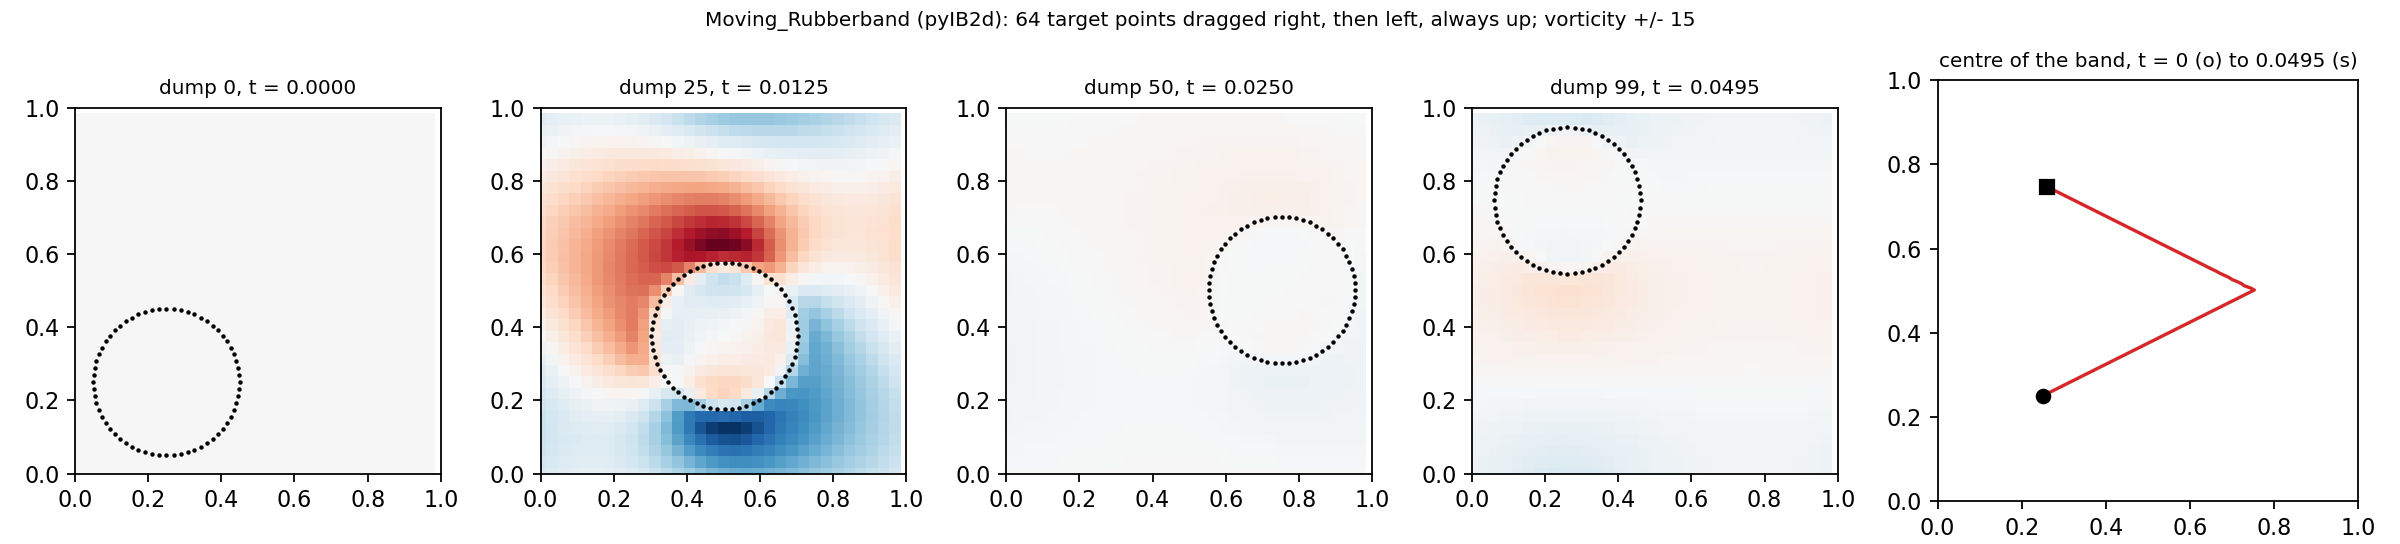
\includegraphics[width=\linewidth,height=0.3\textheight,keepaspectratio]{ch4c-moving-band.png}

\scriptsize\raggedright
\al{Moving\_Rubberband:} a circle of 64 target points (stiffness $10^7$) in viscous fluid on a $32\times32$ grid, dragged along a zig-zag: right then left every 0.05, upward all the time. The targets move by an increment per step; the points follow through the target force. About 3 s; the centre goes from (0.25, 0.25) to (0.75, 0.50) at $t = 0.025$ and ends at (0.26, 0.75).
\column{0.48\textwidth}
\centering
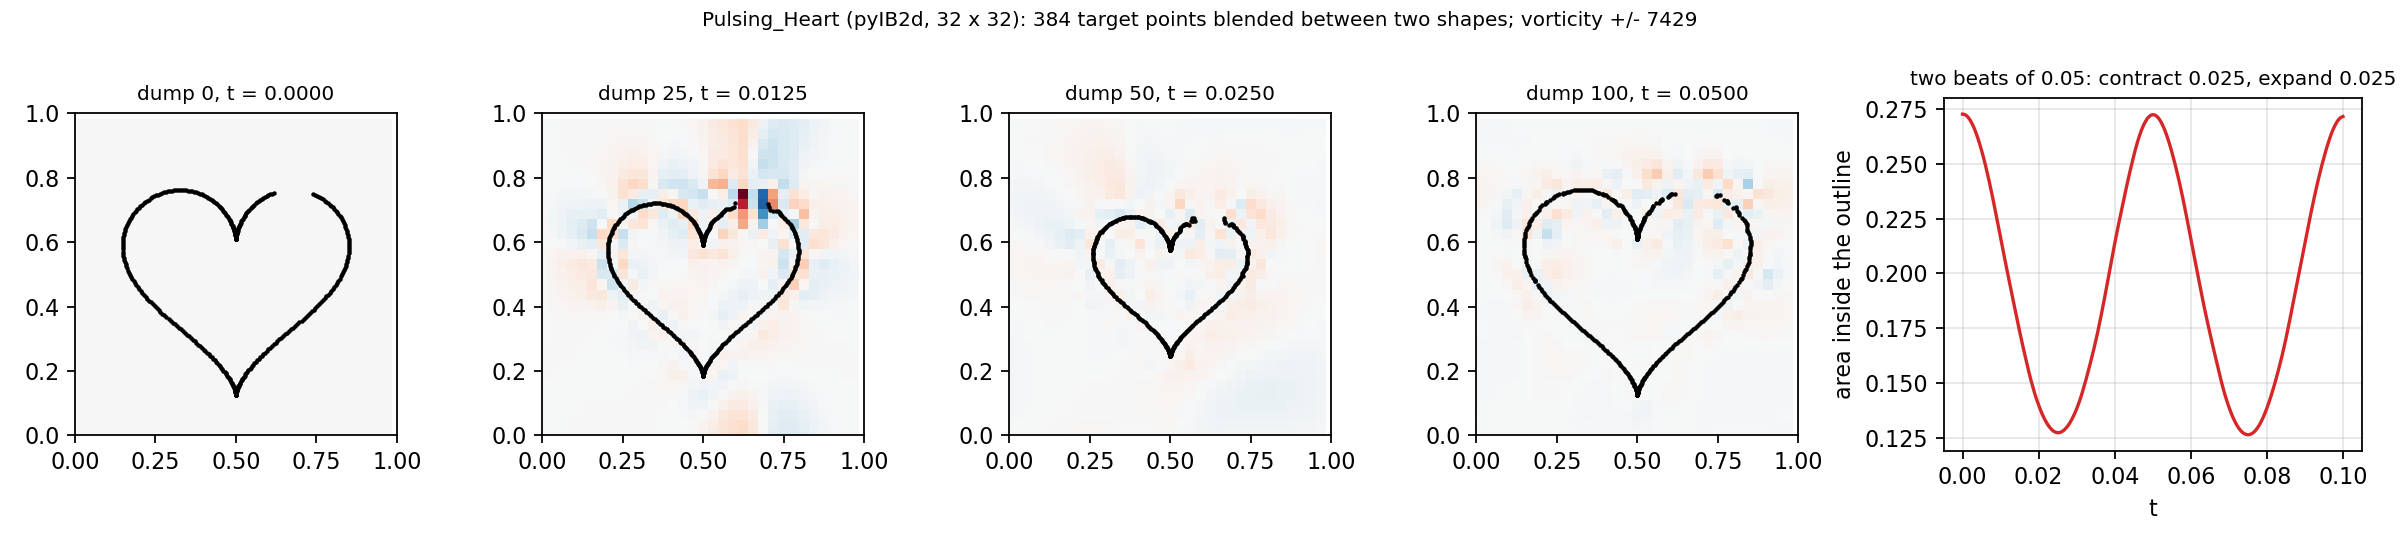
\includegraphics[width=\linewidth,height=0.3\textheight,keepaspectratio]{ch4c-pulsing-heart.png}

\scriptsize\raggedright
\al{Pulsing\_Heart:} a cartoon heart of 384 target points (stiffness $10^8$) whose targets blend between an expanded and a contracted shape, 0.025 each way, starting and ending at rest: the targets as a function of time and of the two stored shapes, so nothing drifts. Two beats in 0.1 (10,000 steps); about half a minute (24 s in chapter 4c), 201 dumps.
\end{columns}
\vspace{1mm}
\footnotesize Both: chapter 4c (the \code{update\_*} functions and their two styles).
\sourcecredit{\code{examples/IB2d/Moving\_Rubberband/README.md}, \code{Pulsing\_Heart/README.md}; ports of IB2d's MATLAB examples.}
\end{frame}

% 29
\begin{frame}{IB2d: Sawtooth}
\label{fr:sawtooth}
\begin{columns}[T,onlytextwidth]
\column{0.42\textwidth}
\expic{ch4c-sawtooth-frames.png}{The teeth and $u_x$ at four dumps of the $256\times64$ run, which fails at $t = 0.12$ (chapter 4c).}
\column{0.55\textwidth}
\scriptsize
\al{What:} two rows of twelve teeth form a channel in a $12\times3$ box; every point is a target point; the top row's targets move down and up as a sine (to the channel's centreline, twice per unit time) and pump (in the MATLAB example; the Python port has not yet run a full cycle). A port of N.~A. Battista's sawtooth pump with the grid, the number of teeth and the box as parameters.

\smallskip
\al{Run:} \code{python3 Sawtooth.py 1024 256} for the original geometry (6552 points), \code{input2d} set to $1024\times256$ and \code{Tfinal = 10}, then \code{main2d.py}: 400,000 steps of $2.5\times10^{-5}$ for the MATLAB example's 10 s (20 cycles), hours.

\smallskip
\al{You should see:} the MATLAB example tethers its points with $k = 10^{11}$ on its full $1024\times256$ grid and runs (its folder holds the flow data of the first three cycles). On the coarser grids tried in Python every run failed with NaN positions before one cycle: \al{this example needs its full grid}.

\smallskip
\al{Chapters:} 4c (moving boundaries, the stiffness-and-grid lesson).
\end{columns}
\sourcecredit{\code{examples/IB2d/Sawtooth/README.md}.}
\end{frame}

% 30
\begin{frame}{IB2d: Stability\_Lab}
\label{fr:stablab}
\begin{columns}[T,onlytextwidth]
\column{0.42\textwidth}
\expic{ch4d-band-map.png}{Stiffness against time step: which runs blow up (chapter 4d).}
\column{0.55\textwidth}
\scriptsize
\al{What:} IB2d's \code{Rubberband\_with\_Springs} with the grid, the stiffness, the resting length and the points per cell as arguments, a sweep script for the chapter's groups of runs, and an analysis script that turns each run's dumps into the band's shape in time.

\smallskip
\al{You should see:} refining the grid (with $k$ and $\Delta t$ scaled) keeps more of the band's area: 79.5\,\% at $16^2$, 87.1\,\% at $32^2$, 95.9\,\% at $256^2$ by $t = 0.98$. On $32^2$ the largest stable $\Delta t$ falls from 0.064 or more ($k = 2.5\times10^3$: every step tried ran) to 0.002 ($2.5\times10^5$); at $2.5\times10^6$ no step size tried ran to the end.

\smallskip
\al{Also:} the shipped band is tall, not wide (the geometry function's arguments are swapped), and has one point per cell, not two.

\smallskip
\al{Chapters:} 4d (stability and convergence: a lab).
\end{columns}
\sourcecredit{\code{examples/IB2d/Stability\_Lab/README.md} (every number on chapter 4d's slides comes from its \code{runs/summary.json} and \code{series.csv} files).}
\end{frame}

% 31
\begin{frame}{IB2d: Muscle\_Models and Mesh\_From\_SVG}
\label{fr:musclesvg}
\begin{columns}[T,onlytextwidth]
\column{0.48\textwidth}
\centering
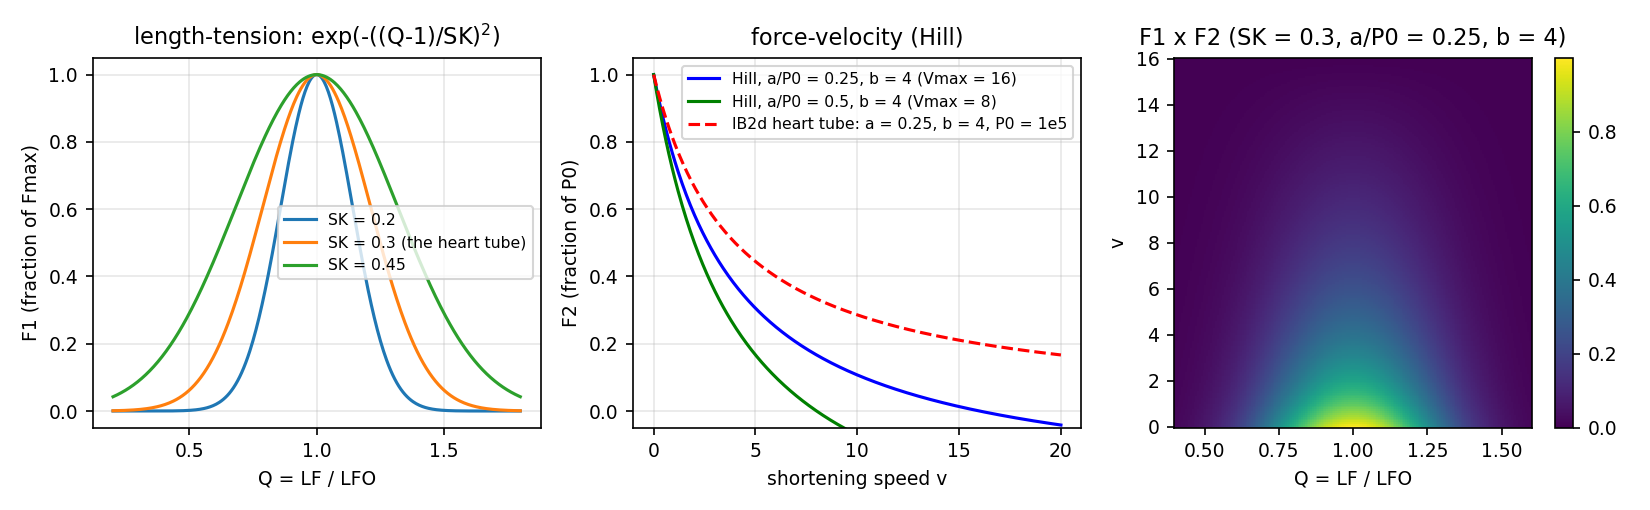
\includegraphics[width=\linewidth,height=0.28\textheight,keepaspectratio]{ch4e-muscle-lt-fv.png}

\scriptsize\raggedright
\al{Muscle\_Models:} three small scripts (NumPy and Matplotlib, no IB2d) that plot and check the muscle laws of chapter 4e: IB2d's force--velocity law against Hill's, a crossbridge model in closed form and by integration (they agree to $4.5\times10^{-8}$ of $P_0$), the heart tube's activation wave, and a calcium model with illustrative rate constants (a twitch peaks at 0.53 after 9 ms; at 100 stimuli per second the response saturates at 1.00).
\column{0.48\textwidth}
\centering
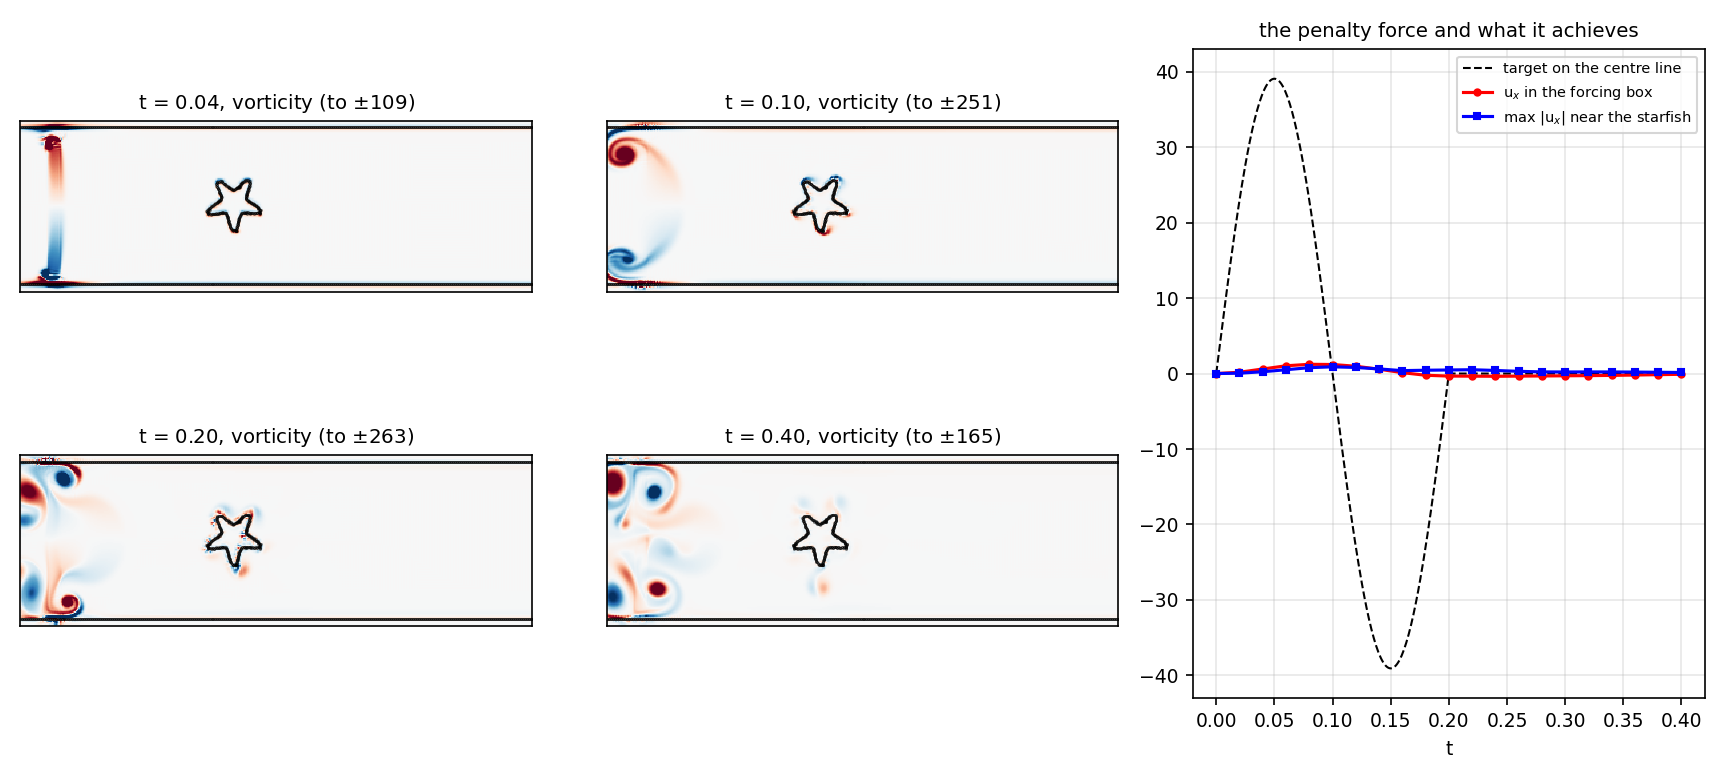
\includegraphics[width=\linewidth,height=0.28\textheight,keepaspectratio]{ch4f-starfish-run.png}

\scriptsize\raggedright
\al{Mesh\_From\_SVG:} \code{svg\_to\_vertex.py}, a sampler that places points $ds = dx/2$ apart along an SVG drawing's paths (as MeshmerizeMe does), and \code{Starfish\_Channel}, IB2d's starfish example in Python at $512\times128$: 405 points on the starfish, walls, a pulsed penalty forcing; 8000 steps in 223 s. Its flow drives chapters 34--35's Planktos examples.
\end{columns}
\vspace{1mm}
\footnotesize Chapters 4e (the model gallery and muscle models) and 4f (meshes from images).
\sourcecredit{\code{examples/IB2d/Muscle\_Models/README.md}, \code{Mesh\_From\_SVG/README.md} and \code{Starfish\_Channel/README.md}.}
\end{frame}

% 32
\begin{frame}{\NoCaseChange{\code{examples/analysis/}}: reading and analysing any run}
\label{fr:analysis}
\scriptsize
\renewcommand{\arraystretch}{0.95}
\begin{tabular}{@{}L{0.33\textwidth}L{0.48\textwidth}L{0.12\textwidth}@{}}
\toprule
scripts & what for & chapters \\
\midrule
\code{hier\_data.py}, \code{read\_hier\_data.m}, \code{leaf\_forces.py/.m}, \code{read\_input.m} & positions and forces from \code{hier\_data\_IB2d}; IB/03's drag and lift; the constants of an input file & 11 \\
\code{samrai\_dumps.py/.m}, \code{read\_vtk\_legacy.py/.m}, \code{read\_exodus.py/.m}, \code{hier\_data\_h5.py} & the fluid and the structure in Python, MATLAB or Octave & 33 \\
\code{flow\_rate.py}, \code{piv\_to\_vtk.py} & flux across a line; PIV data into VTK & 33 \\
\code{visit\_queries.py}, \code{read\_curve.py/.m}, \code{templates/} & averages, picks, lineouts, fluxes through time; \code{.curve} files; the analysis protocol, data sheet and report & 29 \\
\code{visit\_3d.py} & 3D pictures by numbers & 27 \\
\code{visit\_movie\_frames.py}, \code{make\_movie.py}, \code{movie\_clean.py} & frames, an H.264 movie, frames cleaned of level lines & 30 \\
\code{resample\_export.py}, \code{vtk\_for\_planktos.py} & a uniform grid exported to VTK (also with a parallel engine); Planktos's file layout & 33, 32, 31, 35 \\
\code{visit\_frames.slurm} & the frames of a finished run as a Puma batch job (not yet run on Puma) & 31 \\
\bottomrule
\end{tabular}

\vspace{1mm}
\footnotesize The VisIt scripts run inside VisIt's own Python (\code{visit -nowin -cli -s}); the others in any Python 3 with NumPy (h5py, netCDF4 or vtk where a format needs them).
\sourcecredit{\code{examples/analysis/README.md}.}
\end{frame}

% 33
\begin{frame}{\NoCaseChange{\code{examples/Planktos/}} and \NoCaseChange{\code{examples/support/}}}
\label{fr:planktossupport}
\begin{columns}[T,onlytextwidth]
\column{0.44\textwidth}
\centering
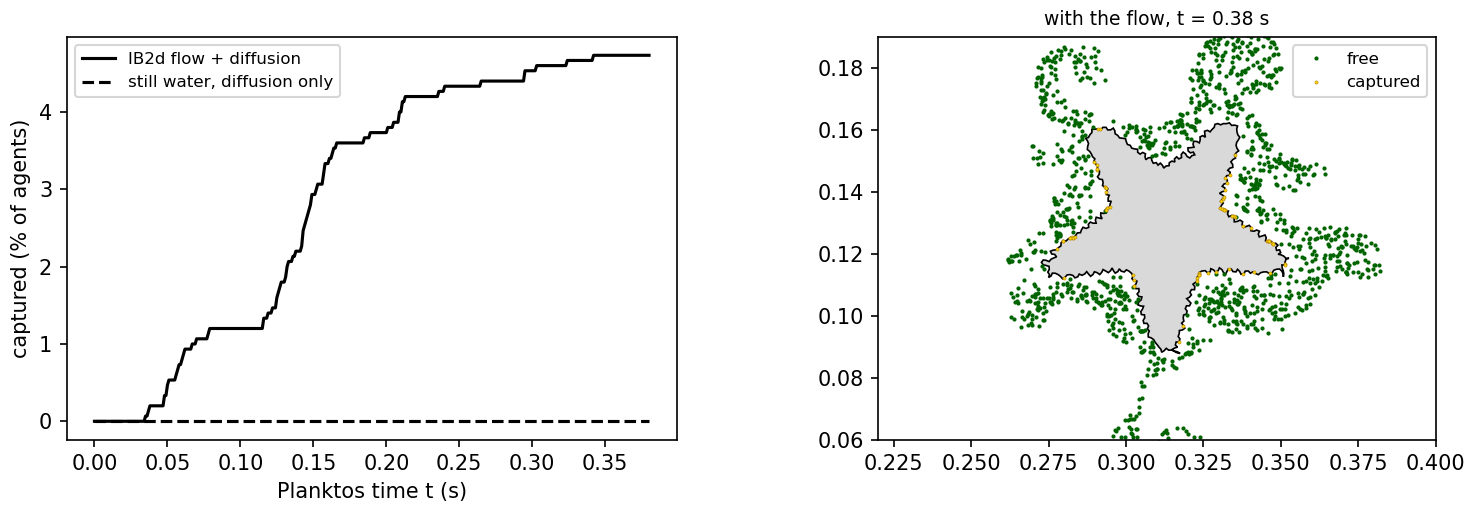
\includegraphics[width=\linewidth,height=0.4\textheight,keepaspectratio]{planktos-starfish-capture.png}

{\tiny\color{DarkGray}Agents captured on the starfish (chapter 35).\par}
\column{0.53\textwidth}
\scriptsize
\al{Planktos (chapters 34, 35):} Planktos 1.0.3 on this series' flows. \code{starfish\_env.py} loads the starfish run of chapter 4f; \code{starfish\_kde.py}, \code{starfish\_capture.py}, \code{starfish\_ftle.py} and \code{starfish\_vicsek.py} release agents in it (density estimates, capture, FTLE maps, alignment); \code{ibamr\_plate.py} takes IBFE/10 through VisIt; \code{brinkman\_first.py} needs no data. Seconds to five minutes each.

\smallskip
\al{support/matlab-exercises (chapters 5, 4d, 16; Appendix A):} the small MATLAB exercises of the course, each with a Python version that does the same thing.

\smallskip
\al{legacy/:} the course example codes as they were, from UNC and the University of Arizona, with the old Makefile build; this catalogue's examples replace them one by one, except one 2020 example folder, which has no successor here.
\end{columns}
\sourcecredit{\code{examples/Planktos/README.md}; \code{examples/support/matlab-exercises/README.md}; the repository's \code{README.md}.}
\end{frame}

% 34
\begin{frame}{Choosing an example to start from}
\label{fr:choose}
\scriptsize
\renewcommand{\arraystretch}{0.95}
\begin{tabular}{@{}L{0.44\textwidth}L{0.5\textwidth}@{}}
\toprule
you want to model & start from \\
\midrule
an elastic body relaxing, the IB basics & IB/01 (IBAMR), IB2d's rubber bands (\code{Stability\_Lab}) \\
a channel or a vessel with an imposed inflow & IB/02 (a straight channel), IB/13 (real vessels, open outflow) \\
a flexible structure in a flow (leaves, hairs, fins) & IB/03 (2D, points); IBFE/10 (3D, finite elements) \\
a body moved by a prescribed motion & IB/04, IB/07 (moving targets); ConstraintIB/01 (rigid) \\
growth, curling, a changing shape & IB/06 (springs), IB/09 (curvature) \\
a body that swims & IB/10 (jellyfish, curvature); ConstraintIB/03 (eel, prescribed deformation) \\
a pump or a heart tube & IB/11 (five actuations); IB2d's \code{Sawtooth} (at its full grid) and \code{Pulsing\_Heart} \\
mass, gravity, falling or sinking & IB/12 (penalty IB); ConstraintIB/02 (a free rigid body) \\
a 3D array or a periodic medium & IB/08 \\
a solid with a real material law or muscle & IBFE/01, 06 (active tension); IB2d's \code{HeartTube\_Muscle} (chapter 4e; the laws plotted in \code{Muscle\_Models}) \\
several bodies & IB/07 (IB), IBFE/08 (IBFE) \\
a dissolved chemical or heat & IBFE/12 \\
organisms carried by the flow & \code{examples/Planktos}: IB2d runs as they are, 3D IBAMR runs through VisIt (chapter 35) \\
\bottomrule
\end{tabular}
\sourcecredit{This chapter's pages; chapter 1b (choosing software and building geometries).}
\end{frame}

% 35
\begin{frame}{Before you change anything}
\label{fr:before}
\footnotesize
\begin{enumerate}\setlength{\itemsep}{2pt}
  \item Run the example unchanged, with the README's core count, and keep the log (\code{tee run.log}).
  \item Compare with ``What you should see'': the \code{integral\{F\}} lines, the table of positions or forces, the number of frames. The READMEs' numbers are the same with IBAMR 0.16.0 and 0.19.0, mostly to the last digit; where a README says a run is sensitive (IB/06's folding, IBFE/06's fourth cycle), small differences from the version, the core count or the machine are normal. A different shape or a stop is not.
  \item Look at it in VisIt the way the README's ``Looking at it in VisIt'' says (chapters 26--28), then measure one number yourself (chapter 29).
  \item Change one thing (a ``Try'' item), predict what it will do, run, compare. Some ``Try'' items break the run on purpose, to show an error message (chapter 16).
  \item Keep each run in its own folder with its input file and a README of what you changed (chapter 29's data sheet).
\end{enumerate}
\begin{punchbox}
\small An example that does not reproduce its README is the first thing to fix: the build, the version, the input file's line endings, or the core count.
\end{punchbox}
\end{frame}

% 36
\begin{frame}{Exercises}
\label{fr:exercises}
\footnotesize
\begin{enumerate}\setlength{\itemsep}{2pt}
  \item Run IB/01 and check the width-to-height ratio at $t = 0.4$ and 1 s against the README (chapter 29's tools, or \code{hier\_data.py}).
  \item Pick the example nearest to your own project from slide \ref{fr:choose}; write down which file you will change first and why.
  \item Run IB/03 with and without its \code{.beam} file; describe the difference and find the chapter that explains it.
  \item Run IBFE/01 with each \code{MOTION}; reproduce the tilt of \code{HALF} at $t = 1$.
  \item Run one ``Try'' item that stops with an error on purpose (IB/01's \code{DT}, IBFE/01's \code{HALF} with \code{SHEAR\_MODULUS = 1}, IB/08's \code{TARGET\_VELOCITY}); read the message and the slide on it (chapter 16; chapter 5 for \code{RefineSchedule}).
  \item Run two IB/11 modes at the same time (with \code{mpirun --bind-to none}), and compare their net flow per period across the tube (chapter 29).
  \item Release Planktos agents in a run of your own (chapter 35's routes: an IB2d run as it is, a 3D IBAMR run through VisIt).
\end{enumerate}
\end{frame}

% 37
\begin{frame}{Summary}
\label{fr:summary}
\begin{itemize}\setlength{\itemsep}{3pt}
  \item 12 IBAMR examples (IB/01--13, no IB/05), 6 IBFE, 3 ConstraintIB, 6 IB2d folders, and the \code{analysis}, \code{Planktos} and \code{support} folders: each with a README that says what to expect.
  \item Every IBAMR example builds the same way (CMake, \code{mpirun}, or \code{sbatch job.slurm}); the IB2d ones run from an IB2d clone's \code{pyIB2d/Examples}.
  \item Run unchanged, compare, then change one thing.
\end{itemize}
\begin{punchbox}
\small The examples are where the chapters meet: each page above names the chapters that explain it.
\end{punchbox}
\end{frame}

% 38
\begin{frame}{References and credits}
\label{fr:refs}
\footnotesize
\begin{itemize}\setlength{\itemsep}{2pt}
  \item This repository's \code{examples/} folders and their \code{README.md} files (October 2026); the pictures are those of the chapters named on each page and IB/13's own.
  \item IB2d: N. A. Battista, A. J. Baird and L. A. Miller, \emph{Integr.\ Comp.\ Biol.}\ 55 (2015) 901--911; N. A. Battista, W. C. Strickland and L. A. Miller, \emph{Bioinspir.\ Biomim.}\ 12 (2017) 036003; N. A. Battista et al., \emph{Math.\ Methods Appl.\ Sci.}\ 41 (2018) 8455--8480; \url{https://github.com/nickabattista/IB2d} (GPL-3.0).
  \item MeshmerizeMe: D. M. Senter et al., \emph{Bioinspir.\ Biomim.}\ 16 (2021) 016008; \url{https://github.com/dmsenter89/MeshmerizeMe}.
  \item IBAMR: \url{https://ibamr.github.io}; autoibamr; the upstream examples (chapters 15 and 25).
  \item Constraint IB: A. P. S. Bhalla, R. Bale, B. E. Griffith and N. A. Patankar, ``A unified mathematical framework and an adaptive numerical method for fluid--structure interaction with rigid, deforming, and elastic bodies,'' \emph{J. Comput.\ Phys.}\ 250 (2013) 446--476.
  \item Planktos: W. C. Strickland et al., \emph{Bull.\ Math.\ Biol.}\ 84 (2022) 72; \url{https://github.com/mountaindust/Planktos} (GPL-3.0).
\end{itemize}
\end{frame}

\end{document}
